% !TeX program = xelatex
\documentclass[12pt,spanish,letterpaper,oneside]{article}
\PassOptionsToPackage{es-noshorthands}{babel}
\def\documenttitle{Ultraestructura, dinámica biosintética y reprogramación molecular de la célula plasmática}
\def\documentsubtitle{Artículo de revisión científica sobre los mecanismos de diferenciación, secreción de anticuerpos y nichos de supervivencia}
\def\documentsubject{Producto Integrador de Aprendizaje (PIA) - Biología Celular}
\def\documentauthor{Carlos Mauricio Carvajal Coronado}
\def\coursename{Biología Celular}
\def\coursecode{REF\#261013755061}
\def\universityname{Universidad Autónoma de Nuevo León}
\def\universityfaculty{Facultad de Agronomía}
\def\universitydepartment{Ingeniero Agrónomo}
\def\universitydepartmentimage{departamentos/logos-institucionales.pdf}
\def\universitydepartmentimagecfg{height=2.1cm}
\def\universitylocation{General Escobedo / Marín, Nuevo León, México}
\def\authortable{%
	\begin{Form}
	\begin{tabular}{@{}ll@{}}
		\textbf{Estudiante:} & Carlos Mauricio Carvajal Coronado\\[0.35cm]
		\textbf{Matrícula:} & 1977875\\[0.35cm]
		\textbf{Modalidad:} & Artículo de revisión científica (100\% escrito)\\[0.35cm]
		\textbf{Docente:} & Dr. Miguel Ángel Dector Carrillo\\[0.35cm]
		\textbf{Unidad de Aprendizaje:} & Biología Celular (PIA - 35 Pts)\\[0.5cm]
		\multicolumn{2}{l}{Fecha de realización: 4 de noviembre de 2026}\\
		\multicolumn{2}{l}{\universitylocation}
	\end{tabular}
	\end{Form}
}

\usepackage{fontspec}
\setmainfont{Arial}
\setsansfont{Arial}
\AddToHook{file/config.tex/after}[aulatex-biologia-celular]{%
  \def\documentfontsize{12}
  \def\documentinterline{1}
  \def\documentparindent{0}
  \def\documentparskip{5}
  \def\fontdocument{custom}
  \def\fonttypewriter{custom}
  \def\stylecitereferences{custom}
  \def\portraitstyle{style1}
  \def\hfstyle{style1}
  \def\hfwidthwrap{true}
  \def\hfwidthtitle{0.44}
  \def\hfwidthcourse{0.52}
  \def\predocpageromannumber{false}
  \def\pagemarginleft{2.5}
  \def\pagemarginright{2.5}
  \def\pagemargintop{2.5}
  \def\pagemarginbottom{2.5}
  \def\firstpagemargintop{3.8}
  \def\sectionfontsize{\large}
  \def\sectionspacingtop{8}
  \def\sectionspacingbottom{4}
  \def\ssectionfontsize{\normalsize}
  \def\ssectionspacingtop{6}
  \def\ssectionspacingbottom{3}
  \def\defaultimagefolder{UANL/ingeniero-agronomo/biologia-celular/img/}
  \def\usepdfmetadata{false}
}
% Template:     Informe LaTeX
% Documento:    Núcleo del template
% Versión:      DEV
% Codificación: UTF-8
%
% Autor: Pablo Pizarro R.
%        pablo@ppizarror.com
%
% Manual template: [https://latex.ppizarror.com/informe]
% Licencia MIT:    [https://opensource.org/licenses/MIT]

% -----------------------------------------------------------------------------
% CONFIGURACIONES
% -----------------------------------------------------------------------------
% Definiciones previas
\input{src/defs}

% Ajustes usuario
\input{src/config}

% -----------------------------------------------------------------------------
% IMPORTACIÓN DE LIBRERÍAS
% -----------------------------------------------------------------------------
\input{src/env/imports}

% -----------------------------------------------------------------------------
% IMPORTACIÓN DE FUNCIONES Y ENTORNOS
% -----------------------------------------------------------------------------
\input{src/cmd/core}
\input{src/cmd/math}
\input{src/cmd/equation}
\input{src/cmd/image}
\input{src/cmd/title}
\input{src/cmd/other}
\input{src/cmd/column}
\input{src/env/environments}

% -----------------------------------------------------------------------------
% IMPORTACIÓN DE ESTILOS
% -----------------------------------------------------------------------------
\input{src/style/code}
\input{src/style/other}

% -----------------------------------------------------------------------------
% CONFIGURACIÓN INICIAL DEL DOCUMENTO
% -----------------------------------------------------------------------------
\input{src/cfg/init}

% -----------------------------------------------------------------------------
% PORTADA
% -----------------------------------------------------------------------------
\input{src/page/portrait}
\input{src/page/portrait_config}

% -----------------------------------------------------------------------------
% CONFIGURACIÓN DE PÁGINA Y ENCABEZADOS
% -----------------------------------------------------------------------------
\input{src/cfg/page}

% -----------------------------------------------------------------------------
% TABLA DE CONTENIDOS - ÍNDICE
% -----------------------------------------------------------------------------
\input{src/page/index}

% -----------------------------------------------------------------------------
% CONFIGURACIONES FINALES
% -----------------------------------------------------------------------------
\input{src/cfg/final}

\RemoveFromHook{file/config.tex/after}[aulatex-biologia-celular]

% -----------------------------------------------------------------------------
% Control de composición anti-huecos, paginación de cierres (Conclusiones y
% Referencias en página nueva independiente) y entorno reutilizable AulatexTable
% (modo encapsulado [\linewidth] y modo multipágina [breakable] con xltabular).
% Requisito editorial del usuario (alcance: materia biologia-celular / carrera).
% -----------------------------------------------------------------------------
\hfuzz=0.5pt
\vfuzz=0.5pt
\renewcommand{\topfraction}{0.90}
\renewcommand{\bottomfraction}{0.85}
\renewcommand{\textfraction}{0.07}
\renewcommand{\floatpagefraction}{0.85}
\renewcommand{\dbltopfraction}{0.90}
\renewcommand{\dblfloatpagefraction}{0.85}
\setcounter{topnumber}{3}
\setcounter{bottomnumber}{2}
\setcounter{totalnumber}{4}
\widowpenalty=10000
\clubpenalty=10000
\raggedbottom

\RequirePackage{etoolbox}
\RequirePackage{placeins}
\RequirePackage{needspace}
\RequirePackage{array}
\RequirePackage{ragged2e}
\RequirePackage{tabularx}
\RequirePackage{longtable}
\RequirePackage{xltabular}
\RequirePackage{booktabs}
\RequirePackage{adjustbox}

\ExplSyntaxOn
\cs_if_exist:NF \aulatexCheckSectionPagebreak
  {
    \cs_new_protected:Npn \aulatexCheckSectionPagebreak #1
      {
        \exp_args:Nnx \regex_match:nnTF { (?i) \A \s* conclusi } { \tl_to_str:n {#1} }
          { \clearpage }
          { \FloatBarrier \needspace{5\baselineskip} }
      }
  }
\ExplSyntaxOff

\makeatletter
\TX@delta=0.5pt
\@ifundefined{NC@rewrite@Z}{%
  \newcolumntype{Z}{>{\raggedright\let\newline\\\arraybackslash\hspace{0pt}}X}%
}{}
\@ifundefined{ifaulatexbreakabletable}{\newif\ifaulatexbreakabletable}{}
\@ifundefined{aulatextablewidth}{\newlength{\aulatextablewidth}}{}
\@ifundefined{AulatexTable}{%
  \newenvironment{AulatexTable}[1][\linewidth]{%
    \par\addvspace{0.20cm}%
    \setlength{\emergencystretch}{2em}%
    \TX@delta=0.5pt%
    \ifstrequal{#1}{breakable}{%
      \aulatexbreakabletabletrue%
      \setlength{\aulatextablewidth}{\linewidth}%
      \setlength{\linewidth}{\aulatextablewidth}%
      \setlength{\hsize}{\aulatextablewidth}%
      \setlength{\LTleft}{0pt}%
      \setlength{\LTright}{\fill}%
      \setlength{\LTcapwidth}{\linewidth}%
      \setlength{\LTpre}{0.15cm}%
      \setlength{\LTpost}{0.15cm}%
    }{%
      \aulatexbreakabletablefalse%
      \setlength{\aulatextablewidth}{#1}%
      \centering%
      \adjustbox{max width=\aulatextablewidth,center}\bgroup%
      \setlength{\linewidth}{\aulatextablewidth}%
      \setlength{\hsize}{\aulatextablewidth}%
    }%
  }{%
    \ifaulatexbreakabletable%
      \par\addvspace{0.20cm}%
    \else%
      \egroup\par\addvspace{0.20cm}%
    \fi%
  }%
}{}

\pretocmd{\subsection}{\needspace{4\baselineskip}}{}{}

\AtBeginDocument{%
  \@ifundefined{aulatexSectionHookInstalled}{%
    \gdef\aulatexSectionHookInstalled{1}%
    \NewCommandCopy{\aulatexOrigSection}{\section}%
    \RenewDocumentCommand{\section}{s o m}{%
      \aulatexCheckSectionPagebreak{#3}%
      \IfBooleanTF{#1}{%
        \aulatexOrigSection*{#3}%
      }{%
        \IfValueTF{#2}{%
          \aulatexOrigSection[#2]{#3}%
        }{%
          \aulatexOrigSection{#3}%
        }%
      }%
    }%
    \@ifundefined{printbibliography}{}{%
      \preto{\printbibliography}{\clearpage}%
    }%
    \BeforeBeginEnvironment{thebibliography}{\clearpage}%
  }{}%
}
\makeatother

% -----------------------------------------------------------------------------
% Marca de Agua Institucional en Portada para Ingeniero Agrónomo (Facultad de Agronomía UANL)
% Recurso de mayor resolución oficial disponible: UANL/assets-uanl/logo-agronomia.png (313x300px RGBA)
% -----------------------------------------------------------------------------
\RequirePackage{eso-pic}
\providecommand{\careerwatermarkimage}{UANL/assets-uanl/logo-agronomia.png}
\providecommand{\institutionalWatermark}[2][0.08]{%
  \AddToShipoutPictureBG*{%
    \put(0,0){%
      \parbox[b][\paperheight]{\paperwidth}{%
        \vfill
        \centering
        \begin{tikzpicture}[remember picture,overlay]
          \node[opacity=#1,inner sep=0pt] at (current page.center) {%
            \includegraphics[width=0.56\paperwidth]{#2}%
          };
        \end{tikzpicture}%
        \vfill
      }%
    }%
  }%
}

\usepackage{tabularx}
\usepackage{booktabs}
\usepackage{amsmath,amssymb}
\usepackage{tikz}
\usetikzlibrary{babel,arrows.meta,positioning,shapes.geometric}
\usepackage[backend=biber,style=apa,sorting=nyt]{biblatex}
\definecolor{uanlblue}{RGB}{0,55,108}
\definecolor{tableblue}{RGB}{233,240,247}
\definecolor{algogreen}{RGB}{30,100,60}
\definecolor{algoblue}{RGB}{25,75,130}
\def\portraittitlecolor{uanlblue}
\def\sectioncolor{uanlblue}
\def\ssectioncolor{uanlblue}
\def\documenttitlehf{Revisión científica: Célula plasmática y producción de anticuerpos}
\hypersetup{colorlinks=true,linkcolor=uanlblue,urlcolor=uanlblue,citecolor=uanlblue,pdfauthor={Carlos Mauricio Carvajal Coronado},pdftitle={Ultraestructura, dinámica biosintética y reprogramación molecular de la célula plasmática},pdfsubject={Producto Integrador de Aprendizaje - Biología Celular UANL}}
\addbibresource{UANL/ingeniero-agronomo/biologia-celular/biologia-celular.bib}
\newcolumntype{Y}{>{\raggedright\arraybackslash}X}
\setlength{\emergencystretch}{2.5em}

\begin{document}
\hypersetup{pageanchor=false}
\begingroup
\fontsize{14}{17}\selectfont
\renewcommand{\Huge}{\fontsize{14}{17}\selectfont\bfseries}
\renewcommand{\large}{\fontsize{14}{17}\selectfont}
\templatePortrait
\clearpage
\endgroup
\hypersetup{pageanchor=true}
\templatePagecfg
\singlespacing
\setlength{\tabcolsep}{8pt}
\renewcommand{\arraystretch}{1.18}
\begin{center}
	{\fontsize{16}{20}\selectfont\bfseries\color{uanlblue} Ultraestructura, dinámica biosintética y reprogramación molecular de la célula plasmática: de la respuesta inmune humoral a la fisiología celular especializada}\\[0.25cm]
	{\fontsize{13}{16}\selectfont\itshape Artículo de revisión científica sobre los mecanismos de diferenciación, compartimentación de endomembranas, secreción constitutiva de inmunoglobulinas y señalización en nichos de supervivencia}\\[0.4cm]
	{\fontsize{11}{14}\selectfont\textbf{Carlos Mauricio Carvajal Coronado}\quad (Matrícula: 1977875)}\\[0.15cm]
	{\fontsize{10}{13}\selectfont Facultad de Agronomía, Universidad Autónoma de Nuevo León, Campus Ciencias Agropecuarias, General Escobedo / Marín, N.L.}\\[0.15cm]
	{\fontsize{10}{13}\selectfont Unidad de Aprendizaje: Biología Celular \textbar\ Docente: Dr. Miguel Ángel Dector Carrillo}
\end{center}

\vspace{0.4cm}

\begin{abstract}
\noindent\textbf{Resumen:} La célula plasmática (o plasmocito) representa el estadio de diferenciación terminal más altamente especializado del linaje de linfocitos B, adaptada morfológica y metabólicamente para operar como una biofábrica macromolecular dedicada a la síntesis y secreción masiva de inmunoglobulinas (anticuerpos). El presente artículo de revisión examina exhaustivamente la biología estructural, fisiológica y molecular de la célula plasmática. Se analiza su ontogenia a partir del encuentro antigénico en centros germinales o focos extrafoliculares, gobernada por una red de represión y activación transcripcional que silencia la identidad proliferativa de célula B (mediante la inactivación de PAX5 y BCL6) e induce el eje maestro de diferenciación integrado por IRF4, PRDM1/Blimp-1 y la forma empalmada de XBP-1 (XBP-1s). Ultraestructuralmente, la célula experimenta una expansión geométrica de su sistema de endomembranas: el retículo endoplásmico rugoso (RER) se hipertrofia hasta ocupar más del 50\% del volumen citoplasmático en densas cisternas lamelares, coordinado con un aparato de Golgi perinuclear prominente y una reorganización de la heterocromatina nuclear en el patrón clásico de ``rueda de carreta''. Esta intensa carga proteica exige la activación permanente pero controlada de la Respuesta a Proteínas Desplegadas (UPR) mediante los sensores IRE1$\alpha$, PERK y ATF6, junto con chaperonas moleculares (BiP/GRP78, PDI), evitando la muerte por estrés proteotóxico. Finalmente, se abordan las vías de exocitosis constitutiva, el recableado metabólico impulsado por la importación mitocondrial de piruvato y los circuitos de señalización por quimiocinas (pérdida de CXCR5/CCR7 y ganancia de CXCR4) que guían el anclaje de células plasmáticas de larga vida (LLPC) en nichos estromales de médula ósea mediados por CXCL12, APRIL e IL-6, discutiendo sus implicaciones en la inmunología veterinaria y la biotecnología agropecuaria.
\vspace{0.25cm}

\noindent\textbf{Palabras clave:} Célula plasmática; inmunoglobulinas; retículo endoplásmico rugoso; diferenciación celular; Blimp-1; XBP-1; respuesta a proteínas desplegadas; exocitosis constitutiva; nicho estromal.
\end{abstract}

\vspace{0.3cm}

\section{Introducción y contexto biológico}

La inmunidad humoral en los vertebrados mandibulados representa una de las adaptaciones evolutivas más complejas para neutralizar agentes patógenos en los fluidos extracelulares \parencite{alberts2022molecular,abbas2022cellular}. En el núcleo funcional de este sistema se encuentra la \textbf{célula plasmática} (plasmocito), descrita seminalmente por Astrid Fagraeus a mediados del siglo XX como el efector celular exclusivo responsable de la producción y liberación sostenida de anticuerpos específicos \parencite{nutt2015generation}.

A diferencia de su precursor, el linfocito B virgen en reposo —cuya morfología quiescente se caracteriza por una relación núcleo-citoplasma elevada y un metabolismo basal orientado a la vigilancia inmune—, la célula plasmática experimenta una metamorfosis fisiológica radical. Al comprometerse con la diferenciación terminal, abandona permanentemente el ciclo celular mitótico (permaneciendo en fase $G_0$) y se transforma en una biofábrica celular especializada, capaz de traducir, procesar, plegar y secretar entre $10^3$ y $10^4$ moléculas de anticuerpo por segundo por célula \parencite{cenci2008progressive,shapiroshelef2005regulation}.

Para la ciencia agropecuaria y la biotecnología moderna, la comprensión mecanicista de la célula plasmática resulta de capital trascendencia. La salud, bioseguridad y rendimiento productivo en la ganadería intensiva (bovinos, porcinos, aves y ovinos) dependen de la generación de títulos elevados y duraderos de anticuerpos protectores inducidos por programas de vacunación o en la transferencia pasiva de inmunidad calostral materna. Asimismo, la ingeniería de anticuerpos monoclonales y policlonales —herramientas indispensables para el diagnóstico ultrasensible de fitopatógenos virales y bacterianos en cultivos agronómicos— se sustenta en la explotación fisiológica de las vías de secreción y supervivencia de los plasmocitos \parencite{tellier2019plasma}.

La tesis central que plantea y argumenta esta revisión sostiene que la célula plasmática no representa una simple etapa terminal pasiva, sino un sistema dinámico altamente regulado donde la citoarquitectura de endomembranas, la reprogramación bioenergética y la supervivencia están gobernadas por un acoplamiento estricto entre el eje transcripcional Blimp-1/XBP-1s y el circuito citoprotector de la Respuesta a Proteínas Desplegadas (UPR). El propósito de este artículo de revisión es desglosar la ontogenia y el circuito transcripcional inductor, la ultraestructura y compartimentación de organelos, la dinámica metabólica y biosintética de la UPR, las vías de transporte vesicular y los mecanismos de comunicación intercelular en nichos estromales de la célula plasmática, integrando literatura científica actualizada y los criterios formativos de la unidad de aprendizaje de Biología Celular de la Universidad Autónoma de Nuevo León.

\section{Origen ontogenético y reprogramación transcripcional}

La diferenciación de un linfocito B hacia célula plasmática no es un evento estocástico, sino un programa guiado por antígeno que ocurre predominantemente a través de dos rutas anatómicas y funcionales: la vía rápida extrafolicular y la vía folicular del centro germinal \parencite{nutt2015generation}.

\subsection{Microambiente inductivo: del foco extrafolicular al centro germinal}
\begin{enumerate}
	\item \textbf{Respuesta extrafolicular rápida:} Tras el reconocimiento inicial de antígenos multivalentes o señales de receptores tipo Toll (TLR), los linfocitos B activados proliferan en cordones medulares ganglionares o en la pulpa roja esplénica, diferenciándose rápidamente en \textbf{plasmablastos}. Estos plasmablastos son células de vida corta (días a semanas) que generan una primera oleada de anticuerpos de baja afinidad (principalmente IgM), esencial para la contención temprana de la infección.
	\item \textbf{Reacción de centro germinal:} Cuando la activación involucra antígenos proteicos dependientes de células T cooperadoras foliculares ($T_{fh}$), los linfocitos B ingresan a los folículos linfoides y fundan centros germinales. En la zona oscura, proliferan activamente como centroblastos y experimentan \emph{hipermutación somática} de los genes de inmunoglobulinas mediada por la enzima citidina desaminasa inducida por activación (AID). Posteriormente, en la zona clara, los centrocitos son seleccionados por su afinidad frente al antígeno retenido en las células dendríticas foliculares (FDC) y reciben señales coestimulatorias críticas por parte de los linfocitos $T_{fh}$ (vía CD40L--CD40 y secreción de IL-21 e IL-4). Aquellas células con mutaciones de máxima afinidad y cambio de isotipo (IgG, IgA, IgE) son instruidas para diferenciarse hacia células plasmáticas de larga vida (\emph{Long-Lived Plasma Cells}, LLPC) o células B de memoria \parencite{tellier2019plasma,abbas2022cellular}.
\end{enumerate}

\subsection{El interruptor transcripcional maestro}
La transición de una célula B que presenta antígeno a una célula secretora involucra un cambio mutuamente excluyente entre dos redes reguladoras génicas antagonistas \parencite{shapiroshelef2005regulation}:

\begin{figure}[htbp]
\centering
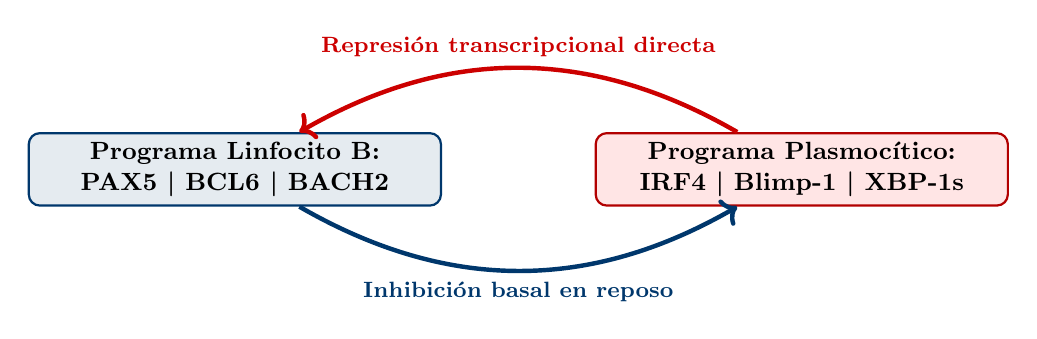
\begin{tikzpicture}[node distance=2.2cm, auto]
\node[draw=uanlblue, thick, rounded corners, fill=uanlblue!10, text width=5cm, align=center, font=\small\bfseries] (bcell) {Programa Linfocito B:\\ PAX5 \textbar\ BCL6 \textbar\ BACH2};
\node[draw=red!70!black, thick, rounded corners, fill=red!10, text width=5cm, align=center, font=\small\bfseries, right of=bcell, xshift=5cm] (plasma) {Programa Plasmocítico:\\ IRF4 \textbar\ Blimp-1 \textbar\ XBP-1s};

\draw[->, ultra thick, red!80!black] (plasma) to [bend right=30] node[above, font=\footnotesize\bfseries, text=red!80!black] {Represión transcripcional directa} (bcell);
\draw[->, ultra thick, uanlblue] (bcell) to [bend right=30] node[below, font=\footnotesize\bfseries, text=uanlblue] {Inhibición basal en reposo} (plasma);
\end{tikzpicture}
\caption{Circuito recíproco de interruptor genético en la diferenciación de células B hacia células plasmáticas.}
\label{fig:circuito_transcripcional}
\end{figure}

\begin{itemize}
	\item \textbf{Factores de identidad de célula B (PAX5, BCL6 y BACH2):} En el linfocito B maduro, el factor PAX5 mantiene la expresión de marcadores de superficie esenciales (CD19, CD20, CD22) y componentes del receptor de célula B (BCR: cadenas accesorias Ig$\alpha$/CD79a e Ig$\beta$/CD79b), reprimiendo simultáneamente los genes efectores de la secreción. Paralelamente, BCL6 reprime la salida del ciclo celular y bloquea la diferenciación terminal para permitir la proliferación clonal en el centro germinal \parencite{nutt2015generation}.
	\item \textbf{Inducción dependiente de la concentración de IRF4:} La estimulación antigénica sostenida incrementa progresivamente los niveles intracelulares del factor regulador de interferón 4 (\textbf{IRF4}). Concentraciones bajas de IRF4 facilitan la proliferación y la expresión de AID, mientras que concentraciones elevadas de IRF4 funcionan como el disparador irreversibe que se une a secuencias reguladoras específicas en los promotores de \emph{Prdm1} y \emph{Xbp1}, forzando la diferenciación plasmocítica \parencite{shapiroshelef2005regulation}.
	\item \textbf{PRDM1 / Blimp-1 (B lymphocyte-induced maturation protein-1):} Es el represor maestro de la célula plasmática. Blimp-1 se une directamente a los promotores de \emph{Pax5}, \emph{Bcl6} y \emph{Myc}, suprimiendo su transcripción. El silenciamiento de PAX5 desencadena la pérdida de los marcadores CD19/CD20 y desacopla la señalización del BCR, mientras que la represión de \emph{Myc} induce la salida permanente del ciclo mitótico y el arresto en fase $G_0$.
	\item \textbf{XBP-1 (X-box binding protein 1):} Mientras Blimp-1 apaga el programa previo, XBP-1 actúa como el activador arquitectónico de la célula secretora. Transcrito por IRF4 y empalmado de manera no convencional a su forma activa hiperestable (\textbf{XBP-1s}) por la endoribonucleasa IRE1$\alpha$, este factor coordina la hipertrofia del retículo endoplásmico, la biogénesis de lípidos de membrana y la inducción masiva de chaperonas moleculares \parencite{todd2009xbp1}.
\end{itemize}

\section{Ultraestructura, compartimentación y organelos especializados}

La adaptación de la célula plasmática a la síntesis masiva de glucoproteínas produce una arquitectura celular única y distintiva entre los tipos celulares de vertebrados \parencite{cenci2008progressive,karp2020cell}.

\subsection{Morfología óptica y ultraestructura microscópica}
Al microscopio óptico con tinción de Wright-Giemsa, la célula plasmática presenta un diámetro medio de 10 a 20 $\mu$m, con una marcada asimetría citoplasmática:
\begin{enumerate}
	\item \textbf{Núcleo excéntrico y cromatina en ``rueda de carreta'':} El núcleo ocupa una posición desplazada hacia la periferia celular. Su característica diagnóstica más sobresaliente es la disposición de grandes bloques electrodensos de heterocromatina adosados a la lámina nuclear interna, alternados radialmente con zonas lúcidas de eucromatina activa, generando el patrón clásico en rueda de carreta o esfera de reloj (\emph{clock-face pattern}). Esta cromatina densa refleja el silenciamiento transcripcional de miles de genes no inmunitarios, concentrando la actividad de transcripción exclusivamente en los loci de cadenas pesadas y ligeras de inmunoglobulinas y genes de soporte secretor \parencite{alberts2022molecular}.
	\item \textbf{Hipertrofia expansiva del Retículo Endoplásmico Rugoso (RER):} El citoplasma muestra una intensa basofilia debido a la saturación de ARN ribosomal. A nivel de microscopía electrónica de transmisión (TEM), el RER deja de ser una red dispersa y se organiza en extensas cisternas paralelas y lamelares que rodean concéntricamente al núcleo y se extienden hasta la corteza subcortical. El RER puede llegar a constituir más del 50\% a 60\% del volumen citoplasmático total \parencite{cenci2008progressive}.
	\item \textbf{Halo claro perinuclear y Complejo de Golgi hipertrofiado:} Adyacente al núcleo excéntrico se observa una zona citoplasmática pálida y negativa a la basofilia, denominada halo perinuclear. La ultraestructura revela que esta región está ocupada por un complejo de Golgi hipertrofiado, compuesto por múltiples pilas de dictiosomas interconectados, enriquecidos en enzimas glicosiltransferasas y vesículas de transporte que procesan las cadenas de anticuerpos antes de su exocitosis.
	\item \textbf{Mitocondrias alargadas y bioenergética:} Dispersas entre las cisternas del RER se localizan numerosas mitocondrias con crestas densas. Estas proveen el suministro continuo de trifosfato de adenosina (ATP) necesario para energizar la translocasa Sec61, la acción de las chaperonas ATPasas de la familia Hsp70 (BiP) y el tráfico vesicular motorizado por dineínas y cinesinas \parencite{lam2018metabolic}.
\end{enumerate}

\begin{table}[htbp]
\centering
\caption{Comparación morfológica, ultraestructural y funcional entre el linfocito B virgen quiescente y la célula plasmática madura.}
\label{tab:comparacion_b_plasma}
\small
\begin{tabularx}{\textwidth}{p{4.2cm}YY}
\toprule
\textbf{Parámetro celular} & \textbf{Linfocito B virgen} & \textbf{Célula plasmática diferenciada} \\
\midrule
Relación Núcleo / Citoplasma & Elevada ($>0.8$), citoplasma escaso & Reducida ($<0.4$), citoplasma abundante \\
Posición y patrón del núcleo & Central; cromatina finamente granular & Excéntrico; heterocromatina en rueda de carreta \\
Volumen relativo del RER & $< 5\%$ del citoplasma; disperso & $> 50-60\%$ del citoplasma; lamelar denso \\
Complejo de Golgi & Rudimentario, difícilmente visible & Hipertrofiado; halo claro perinuclear \\
Estado proliferativo & Capaz de entrar en mitosis ($G_0 \to S$) & Arresto irreversible en fase $G_0$ terminal \\
Receptor de antígeno (BCR) & Alto en membrana (IgM / IgD superficial) & Ausente o residual en superficie \\
Tasa de secreción de anticuerpos & Prácticamente nula ($< 10$ moléculas/h) & Masiva ($10^3 - 10^4$ moléculas/segundo) \\
Marcadores de superficie & $\text{CD19}^+$, $\text{CD20}^+$, $\text{CXCR5}^+$, $\text{B220}^+$ & $\text{CD19}^-$, $\text{CD20}^-$, $\text{CD138}^+$ (Sindecano-1), $\text{CXCR4}^+$ \\
Sensores de estrés UPR & Basales, inactivos & Altamente inducidos y sintonizados \\
\bottomrule
\end{tabularx}
\end{table}

\section{Dinámica biosintética, ensamblaje de anticuerpos y estrés reticular}

El ensamblaje estequiométrico de una molécula de inmunoglobulina monomérica (IgG, por ejemplo) demanda la síntesis y unión covalente coordinada de dos cadenas polipeptídicas pesadas ($\text{H}$) y dos cadenas ligeras ($\text{L}$), formando un heterotetrámero funcional $\text{H}_2\text{L}_2$ estabilizado por puentes disulfuro intercatenarios e intracatenarios \parencite{walter2011unfolded}.

\subsection{Traslocación cotraduccional y control de calidad en el lumen del RER}
Las cadenas $\text{H}$ y $\text{L}$ portan en su extremo amino terminal un péptido señal hidrofóbico. Al emerger del ribosoma en el citosol, es reconocido por la partícula de reconocimiento de la señal (SRP), que detiene temporalmente la elongación y guía al complejo ribosoma-cadena naciente hacia el receptor de SRP en la membrana del retículo. La cadena polipeptídica es enhebrada cotraduccionalmente a través del translocón heterotrimérico \textbf{Sec61} hacia el lumen reticular \parencite{alberts2022molecular,karp2020cell}.

En el interior del retículo:
\begin{enumerate}
	\item La peptidasa de señal escinde el péptido señalizador.
	\item La enzima oligosacariltransferasa transfiere en bloque un oligosacárido precursor ($\text{Glc}_3\text{Man}_9\text{GlcNAc}_2$) a residuos específicos de asparagina presentes en secuencias consenso Asn-X-Ser/Thr (\textbf{N-glicosilación cotraduccional}).
	\item Chaperonas moleculares luminales asisten el plegamiento tridimensional: la proteína de choque térmico \textbf{BiP/GRP78} se asocia transitoriamente a dominios hidrofóbicos expuestos de las cadenas pesadas para prevenir su agregación no específica, reteniéndolas hasta que las cadenas ligeras se sintetizan y desplazan a BiP.
	\item Las enzimas proteína disulfuro isomerasa (\textbf{PDI}) y ERp57 catalizan la formación y reordenamiento oxidativo de los puentes disulfuro esenciales para la conformación globular de los dominios tipo inmunoglobulina.
\end{enumerate}

\subsection{La Respuesta a Proteínas Desplegadas (UPR) como adaptación fisiológica}
Dado que un plasmocito produce millones de enlaces disulfuro y polipéptidos por minuto, el potencial de desbalance y acumulación de intermediarios mal plegados es colosal. Para evitar la toxicidad proteica, la célula plasmática integra de manera permanente la \textbf{Respuesta a Proteínas Desplegadas} (UPR, por sus siglas en inglés) \parencite{walter2011unfolded,cenci2008progressive}:

\begin{figure}[htbp]
\centering
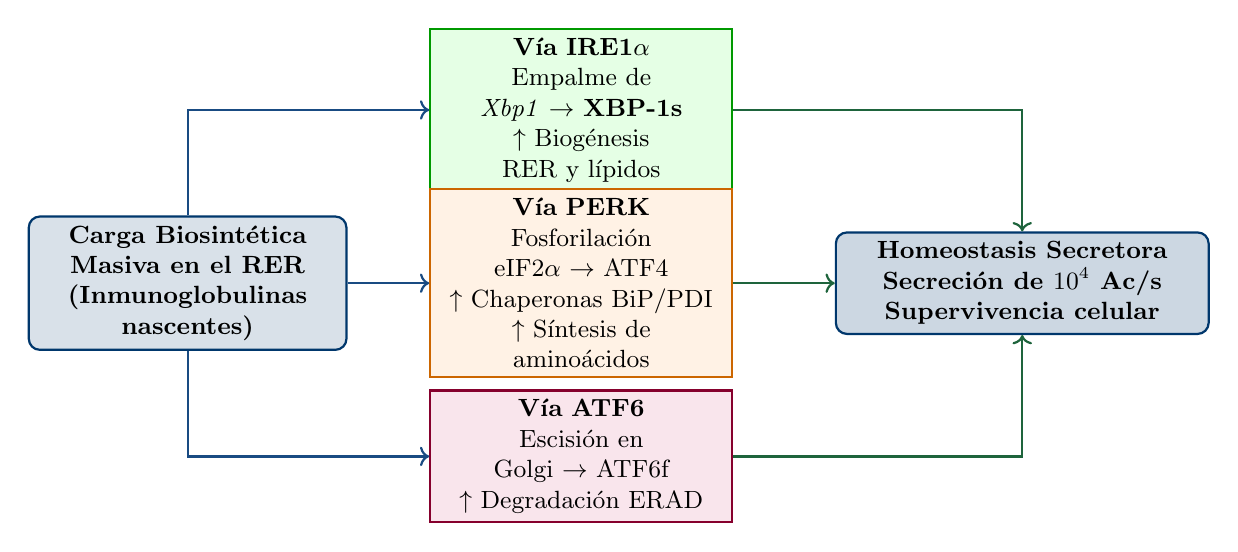
\begin{tikzpicture}[node distance=2.8cm, auto]
\node[draw=uanlblue, thick, rounded corners, fill=uanlblue!15, text width=3.8cm, align=center, font=\small\bfseries] (stress) {Carga Biosintética Masiva en el RER\\ (Inmunoglobulinas nascentes)};

\node[draw=green!60!black, thick, fill=green!10, text width=3.6cm, align=center, font=\small, right of=stress, xshift=2.2cm, yshift=2.2cm] (ire1) {\textbf{Vía IRE1$\alpha$}\\ Empalme de \emph{Xbp1} $\to$ \textbf{XBP-1s}\\ $\uparrow$ Biogénesis RER y lípidos};

\node[draw=orange!80!black, thick, fill=orange!10, text width=3.6cm, align=center, font=\small, right of=stress, xshift=2.2cm] (perk) {\textbf{Vía PERK}\\ Fosforilación eIF2$\alpha$ $\to$ ATF4\\ $\uparrow$ Chaperonas BiP/PDI\\ $\uparrow$ Síntesis de aminoácidos};

\node[draw=purple!70!black, thick, fill=purple!10, text width=3.6cm, align=center, font=\small, right of=stress, xshift=2.2cm, yshift=-2.2cm] (atf6) {\textbf{Vía ATF6}\\ Escisión en Golgi $\to$ ATF6f\\ $\uparrow$ Degradación ERAD};

\node[draw=uanlblue, thick, rounded corners, fill=uanlblue!20, text width=4.5cm, align=center, font=\small\bfseries, right of=perk, xshift=2.8cm] (homeostasis) {Homeostasis Secretora\\ Secreción de $10^4$ Ac/s\\ Supervivencia celular};

\draw[->, thick, algoblue] (stress) |- (ire1);
\draw[->, thick, algoblue] (stress) -- (perk);
\draw[->, thick, algoblue] (stress) |- (atf6);
\draw[->, thick, algogreen] (ire1) -| (homeostasis);
\draw[->, thick, algogreen] (perk) -- (homeostasis);
\draw[->, thick, algogreen] (atf6) -| (homeostasis);
\end{tikzpicture}
\caption{Los tres brazos efectores de la Respuesta a Proteínas Desplegadas (UPR) operando como un circuito homeostático en la célula plasmática.}
\label{fig:upr}
\end{figure}

\begin{itemize}
	\item \textbf{Sensor IRE1$\alpha$ (Inositol-requiring enzyme 1$\alpha$):} Es una endoribonucleasa y quinasa transmembranal del RER. La sobrecarga proteica disocia a BiP de IRE1$\alpha$, permitiendo su oligomerización y autofosforilación. La enzima corta dos sitios específicos en el ARNm inmaduro de \emph{Xbp1}, eliminando un intrón de 26 nucleótidos. Esta alteración del marco de lectura genera el factor de transcripción \textbf{XBP-1s}, el cual transloca al núcleo e induce genes de fosfolípidos (fosfatidilcolina) para expandir la superficie de la bicapa del RER y codifica componentes de degradación asociada al retículo (ERAD) \parencite{todd2009xbp1}.
	\item \textbf{Sensor PERK (Protein kinase RNA-like ER kinase):} Al oligomerizarse, fosforila la subunidad $\alpha$ del factor de iniciación traduccional eucariota 2 (eIF2$\alpha$). Esta fosforilación atenúa transitoriamente la traducción global para desahogar la carga reticular, pero promueve selectivamente la traducción del ARNm de \textbf{ATF4}. ATF4 activa la transcripción de transportadores de aminoácidos, enzimas del metabolismo antioxidante (para mitigar las especies reactivas de oxígeno generadas por la formación de puentes disulfuro) y chaperonas protectoras.
	\item \textbf{Sensor ATF6 (Activating transcription factor 6):} Ante el estrés, ATF6 es transportado mediante vesículas COPII al aparato de Golgi, donde las proteasas S1P y S2P escinden su dominio citosólico. El fragmento soluble resultante (ATF6f) viaja al núcleo para inducir sinérgicamente la síntesis de chaperonas como BiP, calreticulina y enzimas de control de calidad.
\end{itemize}

En las células normales, un estrés no resuelto conduce a la inducción de CHOP y a la apoptosis; sin embargo, las células plasmáticas sintonizan los umbrales de la UPR de modo que los efectores citoprotectores (XBP-1s, BiP) permanezcan crónicamente activos mientras que los inductores de apoptosis son suprimidos activamente por Blimp-1 y Mcl-1 \parencite{walter2011unfolded}.

\section{Tráfico vesicular y mecanismos de secreción constitutiva}

Una vez superados los puntos de control de calidad en el RER, los tetrámeros de inmunoglobulina correctamente ensamblados son empaquetados en vesículas de transporte recubiertas por complejos proteicos \textbf{COPII} (compuestos por Sec23/Sec24 y Sec13/Sec31) en los sitios de salida del retículo endoplásmico (ERES) \parencite{karp2020cell,alberts2022molecular}.

\subsection{Procesamiento en el Complejo de Golgi}
Las vesículas COPII pierden su cubierta y se fusionan homotípicamente para conformar el compartimento intermedio retículo endoplásmico-Golgi (ERGIC), que avanza hacia la red \emph{cis}-Golgi. A medida que las moléculas de anticuerpo avanzan a través de las cisternas \emph{cis}, \emph{medial} y \emph{trans} por progresión de cisternas:
\begin{enumerate}
	\item Las enzimas manoxidasas eliminan residuos de manosa de las cadenas de oligosacáridos unidas a Asn.
	\item Diversas glicosiltransferasas adicionan sucesivamente N-acetilglucosamina (GlcNAc), galactosa, fucosa central y residuos terminales de ácido siálico.
	\item Esta maduración de glucanos en el dominio constante ($F_c$) es biológicamente indispensable: determina la conformación espacial requerida para la interacción del anticuerpo con receptores de superficie celular ($Fc\gamma R$) en macrófagos y neutrófilos, así como para la fijación del primer componente del complemento ($C1q$).
\end{enumerate}

\subsection{Vía secretora constitutiva independiente de gránulos}
A diferencia de las células glandulares endocrinas o exocrinas (como los acinos pancreáticos), que almacenan sus productos en gránulos secretores densos para liberarlos únicamente tras una despolarización o estímulo hormonal (secreción regulada), la célula plasmática madura exhibe una **exocitosis constitutiva continua y no regulada** \parencite{alberts2022molecular}:
\begin{itemize}
	\item Desde la red del \emph{trans}-Golgi (TGN), los anticuerpos procesados son segregados continuamente en vesículas secretoras pos-Golgi sin marcador de retención ni almacenamiento en reservorios intracelulares.
	\item Las vesículas son transportadas a lo largo de filamentos de actina y microtúbulos por proteínas motoras hasta la membrana plasmática.
	\item El anclaje y fusión de las vesículas está orquestado por el complejo de proteínas SNARE: las $v$-SNARE vesiculares interactúan con pares afines de $t$-SNARE (sintaxina y SNAP-25) en la cara citoplásmica de la membrana plasmática, formando un haz de cuatro hélices que aproxima físicamente las bicapas lipídicas y vacía el contenido luminal directamente al fluido intersticial o al estroma tisular.
\end{itemize}

\section{Señalización intercelular, homing y nichos de supervivencia}

Las células plasmáticas se clasifican funcionalmente en dos subpoblaciones discretas que reflejan su ciclo de vida y localización tisular: los plasmablastos de vida corta y las células plasmáticas de larga vida (\emph{Long-Lived Plasma Cells}, LLPC) \parencite{radbruch2006competence}.

\subsection{Recableado de receptores de quimiocinas (Homing a Médula Ósea)}
Para transitar de un plasmablasto migratorio generado en un ganglio linfoide periférico o bazo a una célula residente estable, la célula experimenta una reprogramación estricta de sus receptores de migración (\emph{homing}):
\begin{itemize}
	\item **Pérdida de receptores foliculares:** La supresión de PAX5 apaga la expresión de **CXCR5** (receptor para CXCL13, necesario para la retención en folículos) y **CCR7** (receptor para CCL19/CCL21, que retiene a las células en zonas de linfocitos T).
	\item **Sobreexpresión de CXCR4:** En contraste, la célula incrementa drásticamente la densidad del receptor de quimiocina **CXCR4**. Las células del estroma de la médula ósea y del bazo sintetizan y secretan constitutivamente el ligando quimiotáctico **CXCL12** (SDF-1$\alpha$). El gradiente quimiotáctico de CXCL12 dirige la entrada y arresto de los plasmablastos a través del endotelio vascular hacia los cordones hematopoyéticos de la médula ósea \parencite{radbruch2006competence,tellier2019plasma}.
\end{itemize}

\subsection{Mecanismos moleculares del nicho estromal medular}
En la médula ósea, las células plasmáticas compiten por un número finito de microambientes protectores especializados denominados **nichos multicelulares de supervivencia**, conformados por células estromales reticulares, osteoblastos y eosinófilos residentes \parencite{radbruch2006competence}:

\begin{enumerate}
	\item **Señalización por factores de supervivencia (APRIL y BAFF):** Las células estromales y eosinófilos secretan \textbf{APRIL} (\emph{A Proliferation-Inducing Ligand}) y \textbf{BAFF} (\emph{B-Cell Activating Factor}). La célula plasmática expresa con avidez el receptor **BCMA** (antígeno de maduración de células B / TNFRSF17). La unión de APRIL a BCMA activa la cascada de señalización intracelular dependiente de NF-$\kappa$B, la cual promueve la transcripción continua del gen antiapoptótico **Mcl-1** (de la familia Bcl-2), bloqueando la formación de poros mitocondriales por Bax/Bak y permitiendo la longevidad celular por décadas \parencite{tellier2019plasma}.
	\item **Señalización por Interleucina-6 (IL-6):** La IL-6 liberada en el estroma se une a su receptor heteromérico (IL-6R / gp130), activando la vía de transducción JAK-STAT3, la cual potencia de manera sinérgica la actividad promotora de Blimp-1 y refuerza la maquinaria secretora.
	\item **Adhesión a la matriz extracelular:** La interacción mecánica con la matriz estromal está mediada por la integrina $\alpha_4\beta_1$ (VLA-4) presente en el plasmocito, la cual se ancla fuertemente a la molécula de adhesión celular vascular 1 (\textbf{VCAM-1}) expresada en fibroblastos estromales y a fragmentos de fibronectina tisular. Adicionalmente, el proteoglicano de superficie **CD138** (sindecano-1) secuestra ligandos solubles de heparán sulfato, estabilizando el anclaje físico.
\end{enumerate}

\subsection{Bioenergética mitocondrial y transporte de piruvato}
Estudios metabólicos contemporáneos han desmentido la hipótesis histórica de que las células plasmáticas sustentan su fisiología exclusivamente mediante la glucólisis citoplásmica. La biosíntesis y traslocación de anticuerpos requiere un flujo continuo de ATP generado por fosforilación oxidativa. Las LLPC dependen de la expresión del complejo transportador mitocondrial de piruvato (\textbf{MPC1/MPC2}), el cual importa piruvato activamente al estroma mitocondrial para alimentar el ciclo de Krebs, preservando la viabilidad celular a largo plazo aun en condiciones de privación de nutrientes \parencite{lam2018metabolic}.

\section{Conclusiones y transferencia agrobiotecnológica}

En conclusión, la célula plasmática constituye un paradigma indiscutible de especialización citoarquitectónica y coordinación molecular en la biología celular eucariota. Su tránsito desde un linfocito B en reposo hasta una biofábrica secretora ilustra cómo la integración de redes de factores de transcripción antagónicos (PAX5 vs Blimp-1/XBP-1s) desencadena una reprogramación ultraestructural radical: la expansión geométrica del retículo endoplásmico rugoso, la reorientación paranuclear del aparato de Golgi y el acoplamiento homeostático de la Respuesta a Proteínas Desplegadas (UPR) para tolerar flujos proteicos masivos sin sucumbir a la proteotoxicidad.

En este análisis propio de la biología celular del plasmocito, se advierte que la hipertrofia de endomembranas no representa un mero cambio cuantitativo, sino una transformación funcional cualitativa; esto implica una interpretación integradora donde el hallazgo clave reside en el desacoplamiento selectivo de los sensores de estrés apoptóticos y la consolidación de nichos de supervivencia de larga vida dependientes de CXCL12 y APRIL.

\subsection{Transferencia al ejercicio profesional agropecuario y biotecnológico}
En el contexto laboral y profesional de la ingeniería agronómica y la producción pecuaria, la aplicación práctica de estos fundamentos biológicos resulta de enorme impacto:
\begin{enumerate}
	\item \textbf{Optimización vacunal en animales domésticos:} El diseño de adyuvantes inmunológicos modernos (emulsiones lipídicas, agonistas de TLR y nanopartículas) en la medicina veterinaria busca no solo generar plasmablastos circulantes efímeros, sino modular la expresión de CXCR4 y BCMA para reclutar eficientemente células plasmáticas de larga vida hacia los nichos estromales de médula ósea en ganado bovino, porcino y equino, confiriendo protección vitalicia contra enfermedades endémicas.
	\item \textbf{Biotecnología de anticuerpos recombinantes para la sanidad vegetal:} La ingeniería molecular de líneas celulares derivadas de plasmocitos (mielomas e hibridomas) constituye la piedra angular para sintetizar anticuerpos monoclonales con especificidad antigénica estricta. Estos reactivos biológicos se emplean hoy en pruebas de inmunoensayo ligadas a enzimas (ELISA) y tiras reactivas de flujo lateral para la detección temprana de virus fitopatógenos (como el virus del mosaico del tabaco o el virus de la tristeza de los cítricos) y bacterias cuarentenarias en semillas y plántulas comerciales.
	\item \textbf{Modelado del estrés celular en biofactorías:} La resiliencia del retículo endoplásmico de la célula plasmática frente a la sobrecarga proteica mediante la vía IRE1$\alpha$--XBP-1s ofrece lecciones bioingenieriles directas para diseñar plantas transgénicas y líneas de biofermentación capaces de producir proteínas heterólogas con alto rendimiento sin activar mecanismos celulares apoptóticos.
\end{enumerate}

\newpage

\newpage
\printbibliography[title={Referencias bibliográficas}]
\end{document}
